\message{ !name(2020_EFM_MPM_Eigensoftening.tex)}\documentclass[preprint,12pt,a4paper]{elsarticle}

\usepackage{lineno,hyperref}
\usepackage{float}
\usepackage{subfig}
\usepackage{color}
\usepackage{soul}

\usepackage{algcompatible}
\usepackage{algorithm}
\usepackage{algorithmic}
\usepackage{algpseudocode}

\usepackage{cancel}

\usepackage{amsmath,amsthm,amssymb}
\usepackage{xstring}

\newcommand{\vec}[1]{
  \ensuremath{\mathbf{{#1}}}
}
\newcommand{\tens}[1]{
  \ensuremath{\mathbf{{#1}}}
}
\newcommand{\Matrix}[1]{
  \ensuremath{\mathbf{{#1}}}
}
\newcommand{\Vector}[1]{
  \ensuremath{\mathbf{{#1}}}
}
% Divergence
\newcommand{\Div}[1]{
  \ensuremath{div({#1})}
}
% Gradient
\newcommand\Grad[1]{grad({#1})}
\newcommand\GradS[1]{grad^s({#1})}
\newcommand\GradT[1]{grad^T({#1})}
% Partial derivative
\newcommand{\Deriv}[3][]{
  \ensuremath{\frac{\partial^{#1}{#2}}{ \partial {#3}^{#1} }}
}
% Integral
\newcommand{\Integral}[2]{
  \IfStrEqCase{#1}{
    {2}{\ensuremath{\int_{\varGamma_d}{#2}\ d\varGamma}}
    {3}{\ensuremath{\int_{\varOmega}{#2}\ d\varOmega}}
  }
}


\journal{Engineering Fracture Mechanics}


\modulolinenumbers[5]

%%%%%%%%%%%%%%%%%%%%%%%
%% Elsevier bibliography styles
%%%%%%%%%%%%%%%%%%%%%%%
%% To change the style, put a % in front of the second line of the current style and
%% remove the % from the second line of the style you would like to use.
%%%%%%%%%%%%%%%%%%%%%%%

%% Numbered
%\bibliographystyle{model1-num-names}

%% Numbered without titles
%\bibliographystyle{model1a-num-names}

%% Harvard
%\bibliographystyle{model2-names.bst}\biboptions{authoryear}

%% Vancouver numbered
%\usepackage{numcompress}\bibliographystyle{model3-num-names}

%% Vancouver name/year
%\usepackage{numcompress}\bibliographystyle{model4-names}\biboptions{authoryear}

%% APA style
%\bibliographystyle{model5-names}\biboptions{authoryear}

%% AMA style
%\usepackage{numcompress}\bibliographystyle{model6-num-names}

%% `Elsevier LaTeX' style
\bibliographystyle{elsarticle-num}
%%%%%%%%%%%%%%%%%%%%%%%

\begin{document}

\message{ !name(2020_EFM_MPM_Eigensoftening.tex) !offset(-3) }


\begin{frontmatter}

\title{LME-MPM applied to quasi-brittle fracture.}

%% Group authors per affiliation:
\author{
Miguel Molinos$^a$,
and Pedro Navas$^a$\footnote{Corresponding author: p.navas@upm.es}
 }
 \address{
 $^a$ ETSI Caminos, Canales y Puertos, Universidad Polit\'ectnica de Madrid.\\
 c. Prof. Aranguren 3, 28040 Madrid, Spain
}

\begin{abstract}
  The objective of this work is to introduce an alternative
  technique to address the fracture process of brittle and
  quasi-brittle materials under the material point method (MPM)
  framework. With this purpose the eigensoftening algorithm, developed
  originally for the optimal transportation meshfree (OTM)
  approximation scheme, is extended to the MPM with the aim of present
  a suitable alternative to the existing fracture algorithms developed
  for the MPM. The good fitting in the predictions made by the
  eigensoftening algorithm against both analytical and experimental
  results proofs the well performance of the method under challenging loads.
\end{abstract}

\begin{keyword}
Quasi brittle fracture \sep Local-\textit{max-ent} approximation \sep
Material Point Method \sep Solid Dynamics
\end{keyword}

\end{frontmatter}

\linenumbers

%%%%%%%%%%%%%%%%%%%%%%%%%%%%%%%%%%%%%%%%%%%%%%%%%%%%%%%%%%%%%%%%%%%%%%%%%
\section{Introduction}
\label{sec:1}

The simulation of fracture propagation in a more accurate and
effective way can be considered as one of the original drivers for
developing novel spatial discretization methods such as meshfree
methods like the material point method (MPM). Presence of cracks are a
violation of the continuity requirement of the finite element method
(FEM). To overcome it, numerous of numerical artifacts has been
proposed with the aim of reproduce such a complex behaviour. This
techniques vary from employing cohesive approaches
\cite{Barenblatt,Hilleborg_1976}, by adaptively inserting cohesive
elements \cite{Ortiz_1999,Pandolfi_2002,Ruiz_2000} at solid elements
boundaries, or handling arbitrary cracks paths by level set
representation of the fracture surface \cite{Belytschko_03}.

The severe
limitations of the mesh-dependent methods to simulate fracture
process, have motivated the development of mesh-free technique to
reproduce crack propagation such the element-free Galerkin method
(EFGM) \cite{BELYTSCHKO_1995,BELYTSCHKO_2000,Zhuang_2012,Muthu_2013},
the smoothed particle hydrodynamics (SPH) \cite{Wang_2020,Wang_2019},
the optimal transportation meshfree method (OTM)
\cite{Li2010,Li_2012,Pandolfi_2013,Li_2015} or peridynamics
\cite{HA_2011,RABCZUK_2017}. 

By contrast, MPM does not suffer from the above difficulty since the
continuity requirement is less restrictive. Fracture can be described
in two ways. One is to remove the restriction of the single-valued
velocity field close to the crack by using two or more sets of nodes
\cite{Nairn_2006}. This method is based in to assign different labels
to distinguish if the material points and nodes are in the same side
of the crack or not. Under this approach the crack surface is
described with line segments in 2D and triangle patches in 3D
cases. This method was named as ``CRAcks with Material Points
(CRAMP)'' \cite{Nairn_2003}. In this method, the criteria for crack
propagation is based on such parameters as energy release rate
analyzed by Tan \& Nairn (2002)\cite{Nairn_2002}, and the stress
intensity factor or the J-integral discussed by Guo \& Nairn
(2004)\cite{Nairn_2004}. The other approach is to use failed material
points to describe the crack evolution. In this method, the formation
of failed points describes the nucleation of cracks, and thereafter its propagation and
branching. Consequently, the position of the crack does not need to be
explicitly stated. This represents a significant advantage over the
``CRAMP''. Under this approach, the prediction the failure evolution
employing a decohesion model has been discussed by Chen {\it et al.}\cite{Zhenmao_2005} or
Schreyer {\it et al.}\cite{Schreyer_2002}. And has been successfully
employed to simulate the fracture of brittle materials by Chen {\it et
  al.} \cite{Chen_2002,Chen_2003} and Sulsky \& Schreyer
(2004)\nocite{Sulsky_2004}.


\cite{Belytschko_04,Schmidt_2009,Pandolfi_2012}


The erosion of the material point means that each material point can
be either intact or be completely failed or eroded and has no load
bearing capacity, Even thought the method has been successfully
applied to dynamic fragmentation of metals, quantitative validations,
such as stress or strain levels near or at the crack set compared to
experimental measures are still lacking. Having in mind that the
eigenerosion approach was intended for perfectly brittle fracture, an
eigensoftening concept is developed for quasi-brittle materials

%%%%%%%%%%%%%%%%%%%%%%%%%%%%%%%%%%%%%%%%%%%%%%%%%%%%%%%%%%%%%%%%%%%%%%%%%
\section{The meshfree methodology}
\label{sec:2}

The aim of this section is to provide an overview of the special
techniques employed to face the fracture problem under the MPM
framework. In consequence it is structured as follows: first in
\ref{sec:2.1} the explicit-predictor algorithm for the
MPM will be exposed, next the local \textit{max-ent} approximants are introduced in
\ref{sec:2.2} as an accurate alternative technique to interpolate data
between particles and nodes, and finally the fracture algorithms based
in the eigendeformations are presented in \ref{sec:2.3}.

\subsection{The Material Point Method}
\label{sec:2.1}

The MPM~\cite{Sulsky1994} is a meshfree Lagrangian-Eulerian method
where particles carries on all the physical information and a set of
background nodes is employed to compute the equilibrium
equation. Since the MPM possesses the advantages of both Lagrangian
and Eulerian descriptions, no element distortion exists in the MPM,
therefore it is an appropriate and efficient method in solving
problems involving extremely large deformation and moving
discontinuities such fracture evolution. For the spatial
discretization, two sets of points are introduced in 
the MPM. First, the nodes. This points are considered fixed in the
space and are in charge of computing all the kinematic fields such
forces $f_I$, accelerations $a_I$ and velocities $v_I$. And second the
material points or particles. They are in charge of the discretization
of the continuum, and store the local state ($\sigma_p,
\varepsilon_p$). Without loosing generality, the MPM algorithm
can be described with three main steps: (i) a variational recovery
process, where particle data is projected to the grid nodes, (ii) an
Eulerian step, where balance of momentum equation is expressed as a
nodal equilibrium equation thorough a FEM-like procedure, and finally
(iii) a Lagrangian advection of the particles. In the present research
a explicit predictor-corrector time integration
scheme is adopted. The purpose of this choice is motivated due its proved
robustness and stability in numerical calculations. In the first stage
(i), the nodal velocity predictor is computed following
\eqref{eq:Predictor-velocity}, 
\begin{equation}
  \label{eq:Predictor-velocity}
  \vec{\tilde{v}}_I^{k+1} = \frac{ N_{Ip}^{k} m_p (\vec{v}_p^k + (1 - \gamma)\ \Delta t\ \vec{a}_p^k)}{m_I}
\end{equation}
This way of computing the nodal predictor is both numerically stable
and minimize the computational effort. Once nodal velocity are
obtained, the essential boundary conditions are imposed. And in the
following, a Eulerian phase (ii) is computed in the set of nodes in a
FEM-like way, where nodal forces $\vec{f}_{I}^{k+1}$ are computed thorough the
equilibrium equation. Next the nodal velocities are corrected in a
\textit{corrector} stage,
\begin{equation}
  \label{eq:Corrector-velocity}
  \vec{v}_{I}^{k+1} = \vec{v}_{I}^{pred} + \gamma\ \Delta t\ \frac{\vec{f}_{I}^{k+1}}{\tens{m}_I^{k+1}}
\end{equation}
Finally updated the particles are advected in the Lagrangian stage (iii) using nodal values as,
\begin{align}
  \label{eq:Update-lagrangian-pce}
        &\vec{a}_p^{k+1} = \frac{N_{Ip}^k\vec{f}_{I}^{k}}{\tens{m}_I^k}\\
      &\vec{v}_p^{k+1} = \vec{v}_p^n + \Delta t\
        \frac{N_{Ip}^k\
        \vec{f}_{I}^{k}}{\tens{m}_I^k}\\
      &\vec{x}_p^{k+1} = \vec{x}_p^n + \Delta t\
         N_{Ip}^k\ \vec{v}_{I}^{k} +
        \frac{1}{2}\Delta t^2\ \frac{N_{Ip}^k\
        \vec{f}_{I}^{k}}{\tens{m}_I^k} 
\end{align}
The complete pseudo-algorithm it is summarized in \ref{sec:expl-pred-corr}.

\subsection{Spatial discretization : Local-\textit{max-ent} approximants}
\label{sec:2.2}
Local maximum-entropy (or local \textit{max-ent}) approximation scheme
was introduced by Arroyo \& Ortiz (2006)\cite{Arroyo2006} as a bridge
between finite elements and meshfree methods. The key idea of the
shape functions is to interpret the nodal of a shape function $N_I$ as
a probability. This allow us to introduce two important limits:
maximum-entropy (\textit{max-ent}) limit, and the Delaunay triangulation
which ensures the minimal width of the shape function. The first
limit ensures a \textit{unbiased statistical inference} based on the
nodal data as ensures the Jayne's\cite{Jaynes1957} principle of
\textit{maximum entropy}, the second limit warrant the \textit{least
  width} shape function support. To reach to a compromise between two
competing objectives, a Pareto set is defined as, 
\begin{align*}
  \label{eq:LME-scheme-pareto-set}
  \text{(LME)}_{\beta} \hspace{0.15cm} &\text{For fixed} \hspace{0.15cm}
  \vec{x} \hspace{0.15cm} \text{minimise} \hspace{0.15cm} f_{\beta}(\vec{x}_p, N_I) = \beta U(\vec{x}_p,N_I) - H(N_I) \\
  &\text{subject to}\
  \begin{cases}
    N_I \ge 0, \hspace{0.15cm} \text{I=1, ..., n} \\[1em]   
    \sum\limits_{I=1}^{N_n}{N_I} = 1 \\[1em]   
    \sum\limits_{I=1}^{N_n}{N_I \vec{x}_I} = \vec{x} \\
  \end{cases}
\end{align*}
where $H(N_I)$ is the entropy of the system of nodes following the
definition given by Shannon (1948) \cite{Shannon1948}, and $U(\vec{x}_p,N_I) =
\sum_I N_I |\vec{x}_p - \vec{x}_I |^2$ a 
magnitude of the shape function width. The regularization o
\textit{thermalization} parameter between the two criterion $\beta$
has Pareto optimal values in the range $(0,\infty)$. The unique
solution of the local max-ent problem (LME)$_\beta$ is
 \begin{equation}
  \label{eq:LME-p}
N_I^*(\vec{x})=\frac{\exp\left[ -\beta \; |\vec{x}-\vec{x}_I|^2 +
    \vec{\lambda}^* \cdot (\vec{x}-\vec{x}_I) \right] } {Z(\vec{x},\vec{\lambda}^*)}
\end{equation}
where $Z(\vec{x},\vec{\lambda}^*)$ is the \textit{partition function} defined as,
\begin{equation}
  \label{eq:LME-Z}
Z(\vec{x}, {\vec{\lambda}}) = \sum_{I=1}^{N_n}{ \exp \left[ -\beta \; |\vec{x}-\vec{x}_I|^2 + \vec{\lambda} \cdot (\vec{x}-\vec{x}_I)  \right]}
\end{equation}
and evaluated in the unique minimiser $\vec{\lambda}^*$ for the function $\log
Z(\vec{x}, \vec{\lambda})$. The traditional way to obtain
such a minimiser is using (\ref{eq:LME-J}) to calculate small
increments of $\partial\vec{\lambda}$ in a Newton-Raphson
approach. Where $\tens{J}$ is the Hessian matrix, defined by:
\begin{eqnarray}
  \label{eq:LME-J} 
  \tens{J}(\vec{x}, \vec{\lambda},\beta) &\equiv& \frac{\partial
                                                  \vec{r}}{\partial \vec{\lambda}}\\
  \label{eq:LME-r}
  \vec{r}(\vec{x},\vec{\lambda},\beta) &\equiv& \frac{\partial \log{ Z(   \vec{x},\vec{\lambda}})}{\partial \vec{\lambda}}  = \sum_I^{N_n} p_I(\vec{x},\vec{\lambda},\beta) \, (\vec{x} - \vec{x}_I)
\end{eqnarray}
The value of $\tens{J}$ can be employed to get the first derivatives of the shape function $\nabla
N^*_I$,
\begin{equation}
  \label{eq:LME-grad-p}
\nabla N^*_I = N^*_I  \, \left(\nabla f^*_I-\sum_J^{N_n} N^*_J \, \nabla f^*_J\right)
\end{equation}
where
\begin{equation}
  \label{eq:LME-f}
f^*_I(\vec{x},  \vec{\lambda},\beta)=-\beta \, |\vec{x}-\vec{x}_I|^2 + \vec{\lambda}^*  \,  (\vec{x}-\vec{x}_I)
\end{equation}
Employing the chain rule over \eqref{eq:LME-grad-p}, rearranging and considering $\beta$ as a
constant, Arroyo and Ortiz~\cite{Arroyo2006} obtained the following
expression for the gradient of the shape function.
\begin{eqnarray}
  \label{eq:LME-gradp} 
\nabla N^*_I &=& -N^*_I \,  (\tens{J}^*)^{-1} \,  (\vec{x} - \vec{x}_I)
\end{eqnarray}
The regularization parameter $\beta$ of LME shape functions may be
controlled by adjusting a dimensionless parameter, $\gamma=\beta h^2$
\cite{Arroyo2006}, where $h$ is defined as a measure of the nodal
spacing. Since  $N_I$ is defined in the entire domain, in practice,
the shape function decay $\exp(-\beta \vec{r} )$ is truncated  by  a
given tolerance, 10$^{-6}$, for example,  would ensure a reasonable
range of neighbours, see \cite{Arroyo2006} for details. This tolerance defines
the limit values of the influence radius and is used thereafter to
find the neighbour nodes of a given integration point.

\subsection{Fracture modelling approach}
\label{sec:2.3}
Within the context of MPM formulation, fracture can be modelled by
failing particles according to a suitable criterion. When material
points are failed, they are assumed to have a null stress
tensor. Navas {\it et al.} (2017)\cite{Navas_2017_ES} developed a
eigensoftening algorithm as an extension for quasi-brittle materials
of the eigenerosion proposed by Pandolfi \& Ortiz
(2012)\cite{Pandolfi_2012} for fracture of brittle materials. A
comparison between both in \cite{Navas_2017_ES} shows that
the eigenerosion algorithm significantly overestimates the tensile
stress and the strain peaks, while it captures the forces and crack
patterns accurately. On the other hand eigensoftening algorithm agree
very well with experimental results in all the aspects. Furthermore,
this algorithm has also proof its accuracy for complex fracture
patters such the present in fiber reinforces concrete (FRC),
\cite{Navas_2018_ES}.\\

\begin{align}
  \label{eq:energy-release-EE}
&G_p^{k+1} = \frac{C_{\epsilon}}{m_p^{k+1}}  \sum_{x_q^{k+1} \in
  B_{\epsilon}(x_p^{k+1})} m_q W_q^{k+1}\\
&m_p^{k+1} =  \sum_{x_q^{k+1} \in
  B_{\epsilon}(x_p^{k+1})} m_q  
\end{align}
where $B_{\epsilon}(x_p^{k+1})$ is the sphere of radius $\epsilon$
centered at $x_p^{k+1}$ known as the $\epsilon$-neighborhood of the
material point, $m_p^{k+1}$ is the mass of the neighborhood at step
$k+1$, $W_q^{k+1}$ is the current free-energy density per unit mass as
the material point $x_q^{k+1}$ of the neighborhood, finally
$C_{\epsilon}$ is a normalizing constant. This configuration
conveniently is sketched in Figure \ref{fig:Failed-particles}.
%%%%%%%%%%%
\begin{figure}
  \centering
  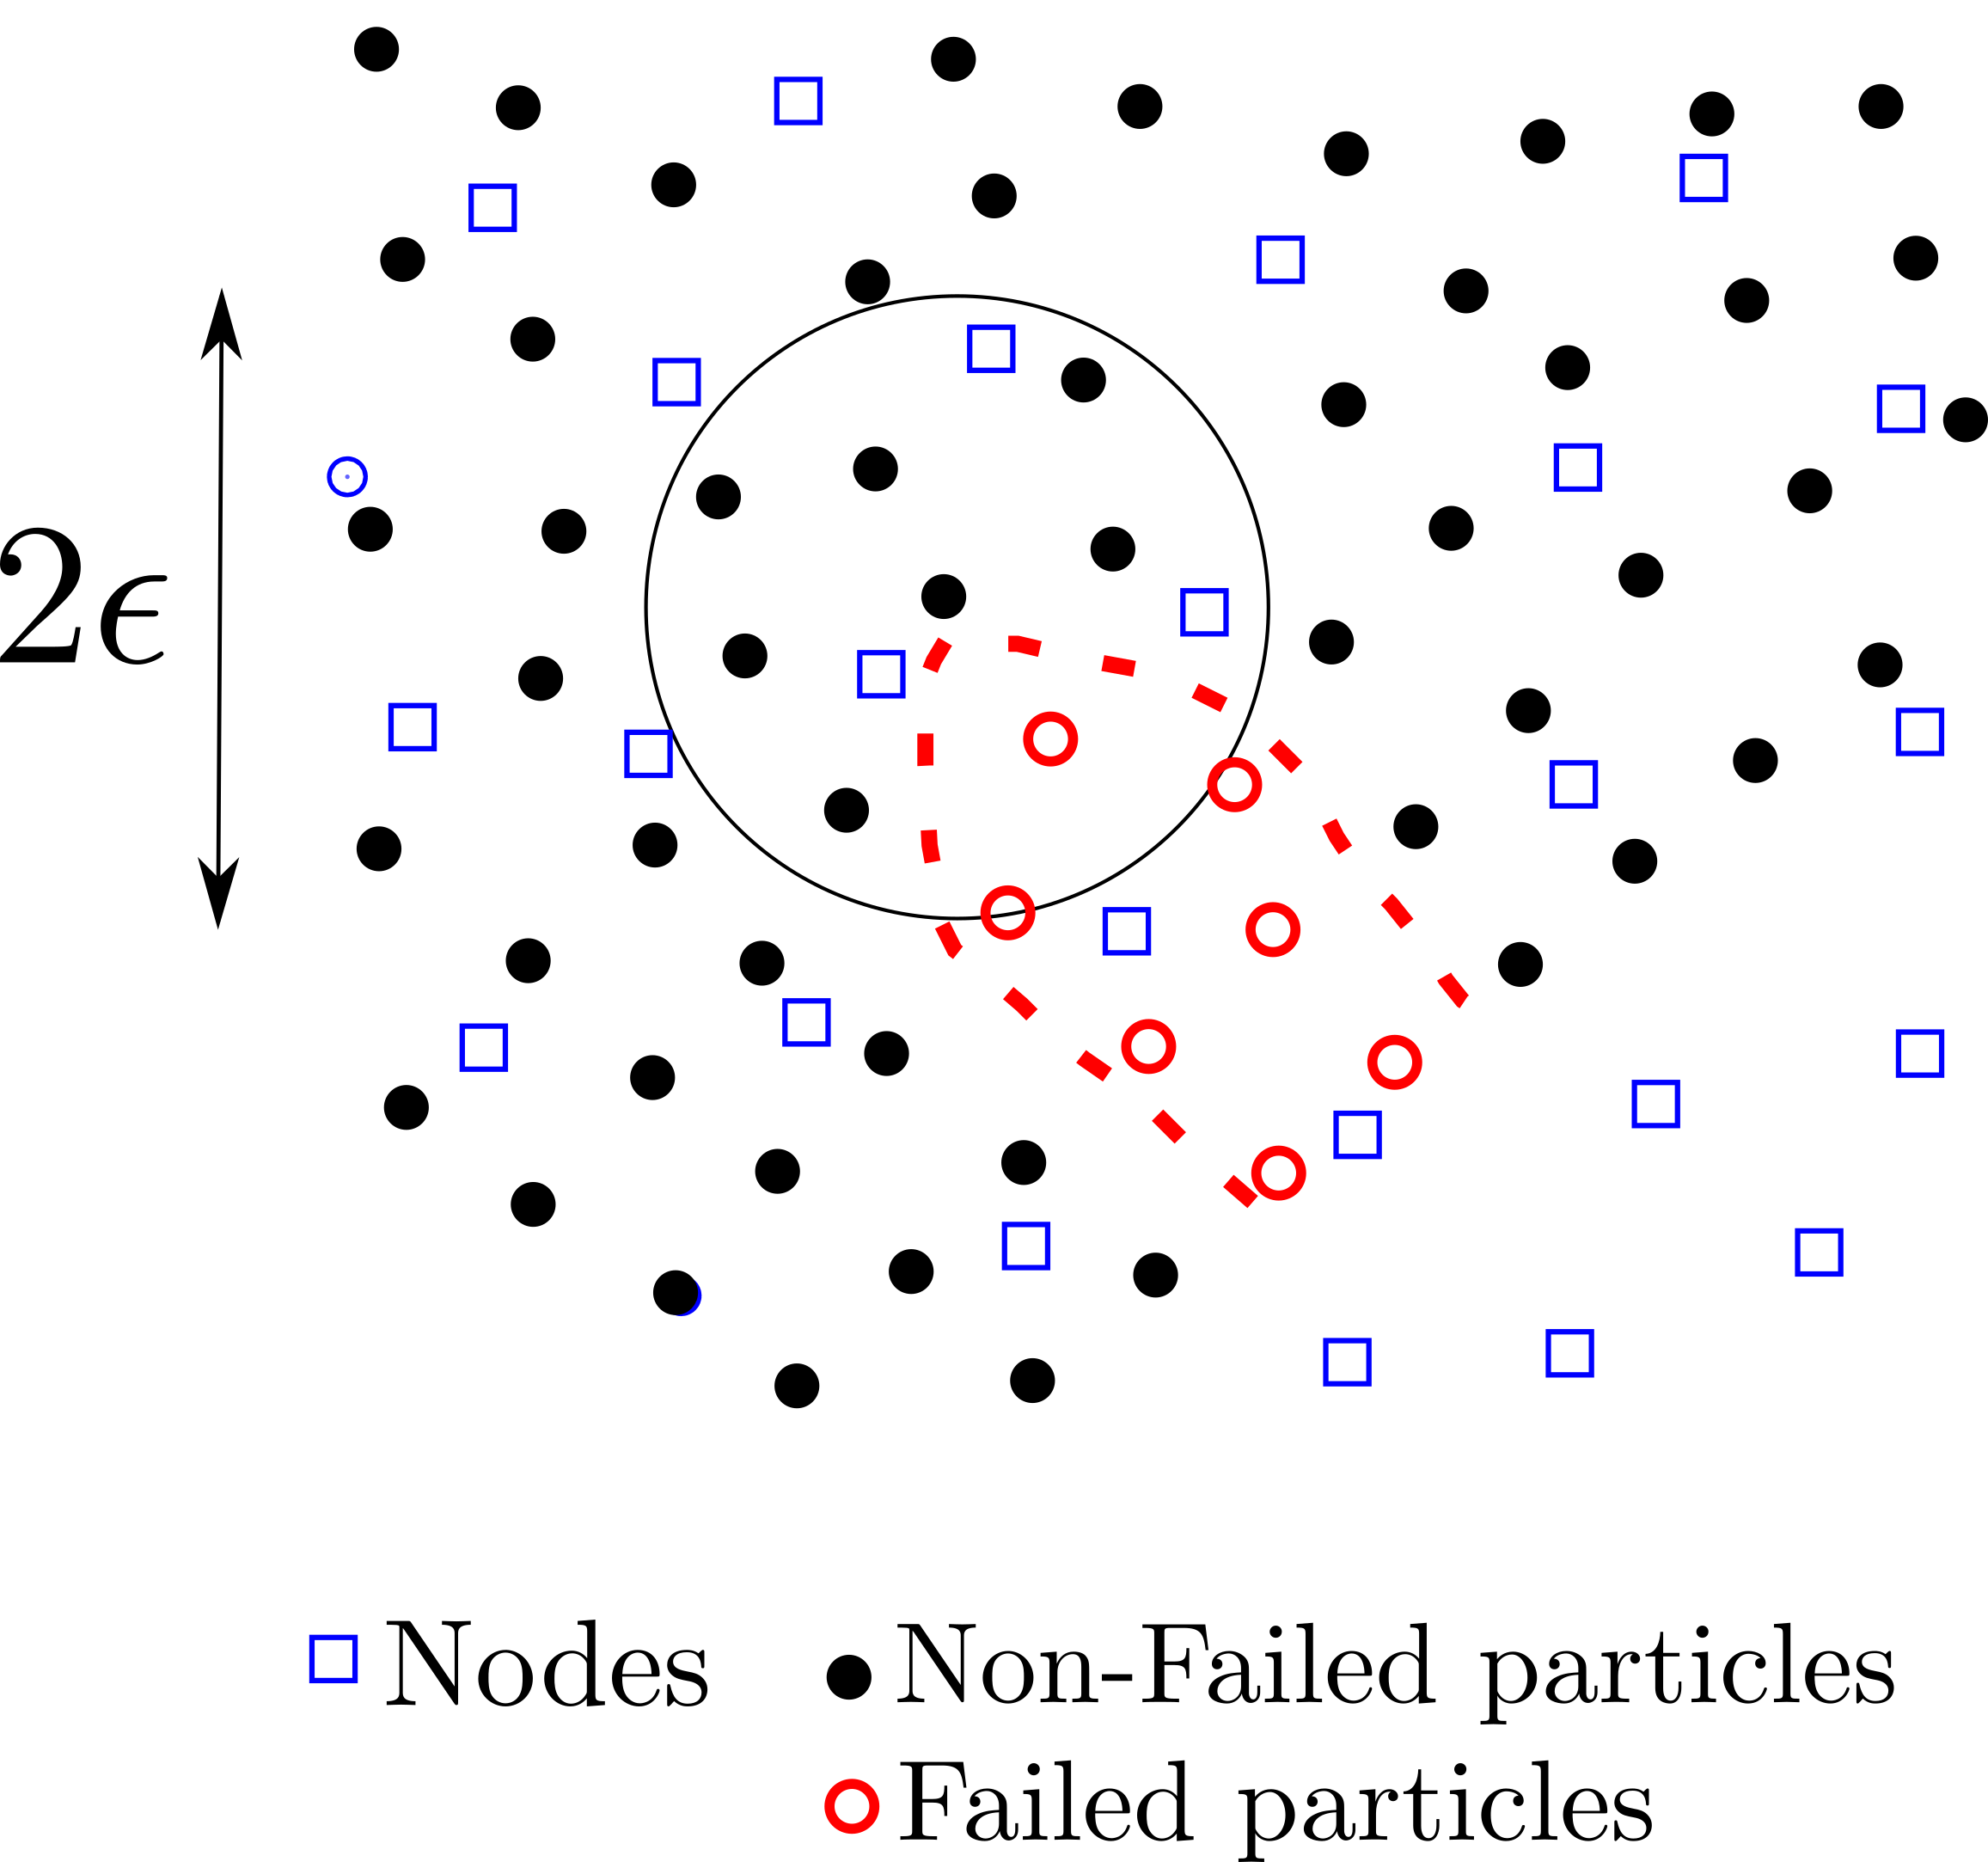
\includegraphics[width=0.5\textwidth]{Figures/Particle-failed}
  \caption{Scheme of a linear cohesive law, where the shaded area is
    $G_f$, $f_t$ is the tensile strength, and $w_c$ is the critical
    opening displacement.}
  \label{fig:Failed-particles}
\end{figure}
%%%%%%%%%%%
The material point fails when $G_p^{k+1}$ surpasses a critical energy
release rate that measures the material-specific energy, $G_F$. The
convergence of this approach has been analyzed by Schmidt {\it et al.}
(2009)\cite{Schmidt_2009}, who proof that it converges to the Griffith
fracture when discretization size tends to zero. It is necessary to
point out that when a material point overpass the critical energy, its
contribution to the internal forces vector  is set to zero, but its
contribution to the mass matrix is maintained. The mass of a material
point is discarded only when an eroded material point is not connected
to any nodes.\\

As can be noticed, in the eigenerosion algorithm an energetic
criterion is adopted. Due to that fact, unrealistic stress
concentration (higher than tensile strength) in quasi-brittle materials, see
\cite{Navas_2017_ES}. To overcome this limitation, the aforementioned
authors proposed the concept of eigensoftening to take in to account
the gradual failure in quasi-brittle materials. The concept is
inspired in the cohesive fracture widely employed in the context of
FEM \cite{Ortiz_1999}. This gradual failure criterion is plotted in
figure \label{fig:Damage-ft-wc}, where a linear decreasing cohesive
law is presented to illustrate the concept here described. In the
picture, the shaded area represents the static fracture energy per
unit of area, $G_F$. Notice how a cohesive crack appears when the
maximum tensile strength, $f_t$ is reached. Once the opening
displacement $w$ takes the value of the critical crack displacement
$w_c$, a stress-free crack is attained. For intermediate values,
$w_n$, a damage value between zero and one represents the extension to
which the material has failed.
%%%%%%%%%%%
\begin{figure}
  \centering
  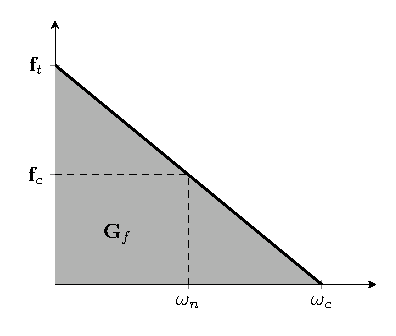
\includegraphics[width=0.5\textwidth]{Figures/Damage}
  \caption{Scheme of a linear cohesive law, where the shaded area is
    $G_f$, $f_t$ is the tensile strength, and $w_c$ is the critical
    opening displacement.}
  \label{fig:Damage-ft-wc}
\end{figure}
%%%%%%%%%%%
For the eigensoftening algorithm, a strength criterion for crack
initialization was adopted. Particularly the maximum principal stress
theory for brittle fracture was considered by authors
\cite{Navas_2017_ES}. With that purpose, the variation of the averaged strain
energy density in the $\epsilon$-neighborhood of the material point
$\vec{x}_p^{k+1}$ can be obtained as,
\begin{equation}
  \label{eq:variation-averaged-strain-energy-density}
  \delta W_{\epsilon,p} = \frac{\partial G_p}{C_{\epsilon}} =
  \frac{1}{m_p} \sum_{x_q^{k+1} \in
  B_{\epsilon}(x_p^{k+1})} m_q \tens{\sigma}_{q,I} \delta \tens{\epsilon}_q
\end{equation}
where $\tens{\sigma}_{q,I}$ is the maximum principal stress of each
material point in the $\epsilon$-neighborhood. Here
\cite{Navas_2017_ES} introduces an effective strain $\varepsilon_q$,
such the variation of the local strain energy can be obtained as
$\delta W_q = \sigma_{q,1} \delta\varepsilon_q$. Now with the assumption
that the effective strain of each material point at every time step
is constant in the neighborhood of $\vec{x}_p^{k+1}$, the equation
\eqref{eq:variation-averaged-strain-energy-density} can be simplified
as follows
\begin{equation}
  \label{eq:variation-averaged-strain-energy-density-simpli}
  \delta W_{\epsilon,p} =
  \frac{\delta \tens{\epsilon}_p}{m_p} \sum_{x_q^{k+1} \in
  B_{\epsilon}(x_p^{k+1})} m_q \tens{\sigma}_{q,I}. 
\end{equation}
Consequently it is possible to define an equivalent critical stress at the
material point $\vec{x}_p^{k+1}$:
\begin{equation}
  \label{eq:equivalent-critical-stress}
  \tens{\sigma}_{\epsilon,p} =
  \frac{1}{m_p} \sum_{x_q^{k+1} \in
  B_{\epsilon}(x_p^{k+1})} m_q \tens{\sigma}_{q,I}, 
\end{equation}
where $m_p$ can be computed as:
\begin{equation}
  \label{eq:averaged-mass}
  m_p = \sum_{x_q^{k+1} \in B_{\epsilon}(x_p^{k+1})} m_q.
\end{equation}
This definition of the equivalent critical stress allow us to
link it with the averaged strain energy as $\delta W_{\epsilon,p} =
 \tens{\sigma}_{\epsilon,p}\ \delta\varepsilon_p$. The fracture
criterion is defined as once $\tens{\sigma}_{\epsilon,p}^{k+1}$
surpasses the tensile strength, $f_t$, the softening behaviour is
activated, which in turn causes a reduction of the initial forces as,
 \begin{equation}
   \label{eq:f-int-damaged}
   f^{int}_I = \sum_p (1 - \chi_p)\ \tens{\sigma}_{p}^{k+1} \cdot \Grad{N_{Ip}}
 \end{equation}
where $\chi_p$ is the damage variable of each material point $p$,
ranges between zero (an intact material) and one (completely failed
material points). For the case of a linear softening such the sketched
in the Figure \ref{fig:Damage-ft-wc}, it is calculated as,
 \begin{equation}
   \label{eq:damaged-variable-chi}
   1 - \chi = \frac{f_n}{f_t} = 1 - \frac{w_n}{w_c}\ \rightarrow\ \chi
   = \frac{w_n}{w_c}.
 \end{equation}
 
Following Bazant~\cite{Bazant83} crack-model, \cite{Navas_2017_ES}
introduced a band width $h_{\epsilon}$, which has values between two
and four times the maximum size of the aggregates for the
concrete. The effective fracture strain $\varepsilon_{\epsilon,f}$ is
defined as the difference between the strain at crack initialization,
$\varepsilon_1(\vec{x}_p^{0})$, and the current strain, $\varepsilon_1(\vec{x}_p^{k+1})$, for material
point $p$. Also, $\varepsilon_{\epsilon,f}$ can be represented as the
current crack opening $w_n$ within the band width,
$h_{\epsilon}$. Therefore,
\begin{equation}
  \label{eq:effective-fracture-strain}
  \varepsilon_{\epsilon,f} = \varepsilon_1(\vec{x}_p^{k+1}) -
  \varepsilon_1(\vec{x}_p^{0}) = \frac{w_n}{h_{\epsilon}}
\end{equation}
Introducing \eqref{eq:effective-fracture-strain} in
\eqref{eq:damaged-variable-chi}, the damage variable can be computed
as,
\begin{equation}
  \label{eq:damage-variable-chi-II}
\chi = \frac{\varepsilon_{\epsilon,f}\ h^{\epsilon}}{w_c}  
\end{equation}
for the case of a linear softening behaviour. In a more general case,
the damage variable can be expressed in terms of the following
variables,
\begin{equation}
  \label{eq:damage-variable-chi-III}
  \chi = \chi(\varepsilon_{\epsilon,f}, h^{\epsilon}, f_t, w_c, G_f)
\end{equation}
%%%%%%%%%%%%%%%%%%%%%%%%%%%%%%%%%%%%%%%%%%%%%%%%%%%%%%%%%%%%%%%%%%%%%%%%%
\section{Cases of study and discussion}
\label{sec:3}

\subsection{Comparison with analytical solution}
\label{sec:3.1}

\subsection{Brazilian test}
\label{sec:3.2}

\begin{figure}
  \centering
  
\includegraphics[width=0.3\textwidth]{Figures/Brazilian}
  \caption{Geometry and boundary condition of the Brazilian test.}
  \label{fig:geometry-brazilian-test}
\end{figure}

\subsection{Drop-weight impact test}
\label{sec:3.3}

\begin{figure}
  \centering
  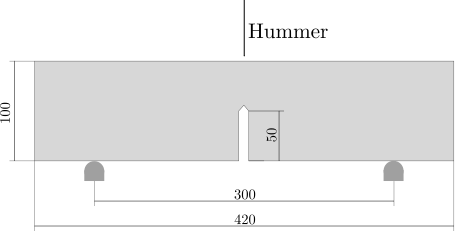
\includegraphics[width=0.8\textwidth]{Figures/Drop_weight}
  \caption{Geometry and boundary condition of the drop-weight impact test.}
  \label{fig:geometry-drop-weight-impact-test}
\end{figure}


%%%%%%%%%%%%%%%%%%%%%%%%%%%%%%%%%%%%%%%%%%%%%%%%%%%%%%%%%%%%%%%%%%%%%%%%%
\section{Conclusions}
\label{sec:6}


\section*{Acknowledgements}
The first author acknowledges the fellowship Agustín de Betancourt 262390106114.

\appendix
%\addappheadtotoc
%\appendixpage
%\renewcommand{\theequation}{\Alph{section}.\arabic{equation}}

\clearpage

\section{Explicit Predictor-Corrector algorithm}
\label{sec:expl-pred-corr}

\begin{algorithm}
  \floatname{algorithm}{Algorithm}
  \renewcommand{\thealgorithm}{}
  \caption{Explicit Predictor-Corrector scheme}
  \begin{algorithmic}[1]
    %%%%%%%%%%%%%%%%%%%%%%%%%%%%%%%%%%%%%%%%%%%%%%%%%%%%%%%%%%%%%%%%%%%%%%%%%%%%%%%%%%%%%% º
    \STATE \textbf{Update mass matrix}:
    \begin{equation*}
      \tens{m}_{I} = N_{Ip}^{k}\ m_p,
    \end{equation*}
    %%%%%%%%%%%%%%%%%%%%%%%%%%%%%%%%%%%%%%%%%%%%%%%%%%%%%%%%%%%%%%%%%%%%%%%%%%%%%%%%%%%%%% 
    \STATE \textbf{Explicit Newmark Predictor}:\\
    \begin{equation*}
      \vec{v}_I^{pred} = \frac{ N_{Ip}^{k} m_p (\vec{v}_p^k + (1 - \gamma)\ \Delta t\ \vec{a}_p^k)}{m_I}
    \end{equation*}
    %%%%%%%%%%%%%%%%%%%%%%%%%%%%%%%%%%%%%%%%%%%%%%%%%%%%%%%%%%%%%%%%%%%%%%%%%%%%%%%%%%%%%% 
    \STATE \textbf{Impose essential boundary conditions}:\\
    At the fixed boundary, set $\vec{v}_{I}^{pred} = 0$. 
    %%%%%%%%%%%%%%%%%%%%%%%%%%%%%%%%%%%%%%%%%%%%%%%%%%%%%%%%%%%%%%%%%%%%%%%%%%%%%%%%%%%%%% 
    \STATE \textbf{Deformation tensor increment calculation}.
    \begin{equation*}
      \Delta \tens{\varepsilon}_{p}^{k+1} = \Delta t\
        \dot{\tens{\varepsilon}_{p}}^{k+1} = \Delta \left[ \vec{v}_{I}^{pred} \otimes
        \Grad{N_{Ip}^{k+1}} \right]^s
    \end{equation*}
    %%%%%%%%%%%%%%%%%%%%%%%%%%%%%%%%%%%%%%%%%%%%%%%%%%%%%%%%%%%%%%%%%%%%%%%%%%%%%%%%%%%%%% 
    \STATE \textbf{Update the density field}:
    \begin{equation*}
      \rho_p^{k+1} = \frac{\rho_p^k}{1 + \mathit{tra}\left[\Delta\tens{\varepsilon}_{p}^{k+1}\right]}.
    \end{equation*}
    %%%%%%%%%%%%%%%%%%%%%%%%%%%%%%%%%%%%%%%%%%%%%%%%%%%%%%%%%%%%%%%%%%%%%%%%%%%%%%%%%%%%%% 
    \STATE \textbf{Compute stress field and update damage parameter}:\\
    %%%%%%%%%%%%%%%%%%%%%%%%%%%%%%%%%%%%%%%%%%%%%%%%%%%%%%%%%%%%%%%%%%%%%%%%%%%%%%%%%%%%%% 
    \STATE \textbf{Balance of forces calculation}:\\
    Calculate the total grid nodal force $\vec{f}_{I}^{k+1} =
    \vec{f}_{I}^{int,k+1} + \vec{f}_{I}^{ext,k+1}$.
    %%%%%%%%%%%%%%%%%%%%%%%%%%%%%%%%%%%%%%%%%%%%%%%%%%%%%%%%%%%%%%%%%%%%%%%%%%%%%%%%%%%%%% 
    \STATE \textbf{Explicit Newmark Corrector}:\\
    \begin{equation*}
      \vec{v}_{I}^{k+1} = \vec{v}_{I}^{pred} + \gamma\ \Delta t\ \frac{\vec{f}_{I}^{k+1}}{\tens{m}_I^{k+1}}  
    \end{equation*}
    %%%%%%%%%%%%%%%%%%%%%%%%%%%%%%%%%%%%%%%%%%%%%%%%%%%%%%%%%%%%%%%%%%%%%%%%%%%%%%%%%%%%%%
    \STATE \textbf{Update particles lagrangian quantities}:
    \begin{align*}
      &\vec{a}_p^{k+1} = \frac{N_{Ip}^k\vec{f}_{I}^{k}}{\tens{m}_I^k}\\
      &\vec{v}_p^{k+1} = \vec{v}_p^n + \Delta t\
        \frac{N_{Ip}^k\
        \vec{f}_{I}^{k}}{\tens{m}_I^k}\\
      &\vec{x}_p^{k+1} = \vec{x}_p^n + \Delta t\
         N_{Ip}^k\ \vec{v}_{I}^{k} +
        \frac{1}{2}\Delta t^2\ \frac{N_{Ip}^k\
        \vec{f}_{I}^{k}}{\tens{m}_I^k}
    \end{align*}
    %%%%%%%%%%%%%%%%%%%%%%%%%%%%%%%%%%%%%%%%%%%%%%%%%%%%%%%%%%%%%%%%%%%%%%%%%%%%%%%%%%%%%% 
    \STATE \textbf{Reset nodal values}
  \end{algorithmic}
\end{algorithm} 


\section{Eigensoftening Algorithm}
\label{sec:eigens-algor-1}

\begin{algorithm}
  \caption{Compute damage parameter $\chi_p^{k+1}$}
  \label{alg-eigens}
  \begin{algorithmic}
    \Require Particle status\\
    Number of particles: $N_p$\\
    $\epsilon$-neighbourhood of each particle $p$ : $B_{\epsilon,p}$\\
    \Require Material data\\
    Tensile strength: $f_{t,p}$\\
    Bandwidth of the cohesive fracture: $h_{\epsilon,p}$ \\
    Critical opening displacement: $w_c$\\ 
    \Ensure Return damage parameter $\chi := \{\chi_p\}$
    \State $\chi_p \leftarrow \chi_p^{k}$
    \For{$p$ to $N_p$}
    \If{$\chi_p = 0$ \AND $\epsilon_{f,p} = 0$}
    \For{$q \in B_{\epsilon,p}$}
    \If{$\chi_q < 1$}    
    \State $\sum m_p\sigma_{p,I} \leftarrow \sum m_p\sigma_{p,I} + m_q\sigma_{q,I}$
    \EndIf    
    \State $m_p \leftarrow m_p + m_q$
    \EndFor
    \State $\sigma_{p,\epsilon} \leftarrow \frac{1}{m_p} \sum m_p\sigma_{p,I}$
    \If{$\sigma_{p,\epsilon} > f_{t,p}$}
    \State $\epsilon_{f,p} = \epsilon_{I,p}$   
    \EndIf        
    \Else[$\chi_p \neq 1$ \AND $\epsilon_{f,p} > 0$]
    \State $\chi_p^{k+1} \leftarrow \min\Big \{1 , \max \{\chi_p^{k},
    \frac{(\epsilon_{I,p}- \epsilon_{f,p})\ h_{\epsilon,p}}{w_c} \} \Big \}$    
    \EndIf    
    \EndFor
  \end{algorithmic}
\end{algorithm}

% name your BibTeX data base
\bibliography{Biblio/Biblio} 

\end{document}
\message{ !name(2020_EFM_MPM_Eigensoftening.tex) !offset(-660) }
